\DocumentMetadata{
  % PDF standards: ONE key whose value is a comma-separated list --
  % UA-2 (accessibility) plus A-4f (archival; the archival companion of
  % UA-2). Do NOT use separate pdfstandard=... keys: with ordinary
  % key-value parsing only the last one takes effect.
  pdfstandard={UA-2,A-4f},
  lang=en-US,
  tagging=on,
  tagging-setup={
    math/setup=mathml-SE
  }
}

\documentclass[addpoints,12pt]{exam}
% quiz-macros.tex -- shared package setup for quiz-template.tex (exam class).
%
% NOTE ON PATHS: every template in this repository is stored one level up
% from where it is compiled (see README.md). All relative \input paths
% below are resolved against the folder the document is compiled in,
% which sits one directory above this file.

\newcommand{\coursename}{[Course, set with CourseName]}
\newcommand{\CourseName}[1]{\renewcommand{\coursename}{#1}}

\newcommand{\timelimit}{[Time Limit, set with TimeLimit]}
\newcommand{\TimeLimit}[1]{\renewcommand{\timelimit}{#1}}

\newcommand{\semester}{[Semester, set with Semester]}
\newcommand{\Semester}[1]{\renewcommand{\semester}{#1}}

\newcommand{\examtype}{[Quiz or Exam, set with IsQuiz or IsExam]}
\newcommand{\IsQuiz}{\renewcommand{\examtype}{quiz}}
\newcommand{\IsExam}{\renewcommand{\examtype{exam}}}

% bm: bold vectors (\bm{v}) for physics-style notation in quiz math.
\usepackage{bm}

% --- exam-class patch: point labels next to each \item ---------------------------
% Redefines exam.cls's internal \item@points@pageinfo so the "N pts" label
% is typeset in a group and inserted into the \@labels box -- the box
% exam.cls uses (since v2.218) to attach page-info to the right \item even
% when a question starts with a list/verbatim environment (those
% environments clobber \everypar, which is why the old approach broke).
% \makeatletter is required so the @-names below resolve; the matching
% \makeatother below restores normal catcodes for the rest of the document.
\usepackage{graphicx}
\usepackage{setspace}
\usepackage{enumitem}
\usepackage{amsmath, amsfonts}
\usepackage[none]{hyphenat} %prevent hyphenation
\makeatletter
\ExplSyntaxOn
\def\item@points@pageinfo{%
  \item 
  \if@placepoints
    \if@bonus
      \def\padded@point@block{%
        \begingroup
          \@placepointstrue
          \bonuspoint@block
        \endgroup
      }%
    \else
      \def\padded@point@block{%
        \begingroup
          \@placepointstrue
          \point@block
        \endgroup
      }%
    \fi
    \if@pointsdropped
      % Do nothing!
    \else
      \if@bonus
        \if@bonusqformat
          \ifx\ques@ref\@queslevel
            % Do nothing
          \else
            \setup@point@toks
          \fi
        \else
          \setup@point@toks
        \fi
      \else
        \if@qformat
          \ifx\ques@ref\@queslevel
            % Do nothing
          \else
            \setup@point@toks
          \fi
        \else
          \setup@point@toks
        \fi
      \fi
    \fi
    \global \@placepointsfalse
  \fi
  % Version 2.218$\beta$, 2007-10-31 changes:
  % Instead of appending
  %   \the \pageinfo@commands \the \point@toks
  % to \everypar, we insert them into the box \@labels.  This corrects
  % the problem that arose when a question (or part, etc.) begins with
  % a list environment (including verbatim, flushleft, center,
  % flushright, and possibly others that are implemented as trivlist
  % environments).  The \item command in those environments throws
  % away the previous contents of \everypar, and so the tokens \the
  % \pageinfo@commands \the \point@toks didn't get inserted where we
  % expected.  List environments *do* preserve the contents of the box
  % \@labels, though.
  \global\setbox\g__block_labels_box\hbox{\unhbox\g__block_labels_box %<----------use new name ...
    \the \pageinfo@commands
    \the \point@toks}%
}
\ExplSyntaxOff
\makeatother

% --- Tagged PDF: table headers -----------------------------------------------------
% Tell tagpdf to mark row 1 of every table as a header row, so screen
% readers announce it as a table header.
\tagpdfsetup{table/header-rows={1}}

% --- Name / Student ID box --------------------------------------------------------------
% Prints the answer instructions plus fill-in lines for Name and Student
% ID at the top of the quiz sheet.
\usepackage{multicol}
\usepackage{tabularx}
\usepackage{lastpage}
\newcolumntype{L}{>{\raggedright\arraybackslash}X}
\makeatletter
\def\@maketitle{%
  \newpage
  \null
  {%
    \setlength{\parindent}{0pt}%

    \begin{tabularx}{\textwidth}{l X}
      \textbf{\coursename} & \textbf{Name:} \hrulefill \\

      \textbf{\semester} & \\

      \textbf{\@title} & \\

      \textbf{\@date} & \\

      \textbf{Time Limit: \timelimit}  & \textbf{Student ID:} \hrulefill
    \end{tabularx}
  }

  \hrule
  \vfill
  \begin{singlespace}
{
  \setlength{\parindent}{0in}

  This \examtype\ consists of \numquestions\ questions across \pageref{LastPage} pages worth \numpoints\ points.

  \textbf{Rules:}
}
\begin{itemize}[nosep]
  \item You have the indicated amount of time above to complete the \examtype\, and you must not begin working on the \examtype\ until instructed to do so.

  \item You must show all of your work to receive full credit, unless stated otherwise. \textbf{On problems that require work to be shown, answers that are mysterious or unsupported will not receive full credit.}

  \item You may not use a calculator, textbook, notes or any other external resources.

  \item Please write your initials at the top of every page in the event the pages become separated.

  \item If you run out of space on a page, feel free to use the back of the page to continue your work.

  \item You understand that if you violate any of these or the University's rules, you will receive a score of zero on this \examtype\, and you may be subject to further disciplinary action.
\end{itemize}

{
  \setlength{\parindent}{0in}
  \vfill
  Following the University of Minnesota’s policy on academic honesty, I pledge that the work shown on this \examtype\ is entirely my own and that I have followed the rules stated above. 

  \vfill
  Signature: \hrulefill
}
\end{singlespace}

\begin{center}
  \pointtable[v][questions]
\end{center}
}
\makeatother
% 4. Reduce space below the Date (before main text)
% --- Points summary ----------------------------------------------------------------------
% "This quiz is worth \numpoints points ... 15 minutes" plus the exam-
% class \pointtable listing the points per question.
\newcommand{\PointsSection}{
  This quiz is worth \numpoints\ points and consists of \numquestions\ questions. You have 5 minutes to complete the quiz.

  \begin{center}
    \pointtable[v][questions]
  \end{center}
}

% --- Math -------------------------------------------------------------------------------
\usepackage{amsmath,amssymb}

% --- Shared course macros ---------------------------------------------------------------
% Root macros.tex: math shorthands used across all course documents
% (\RR, \NN, \ZZ, \QQ, \grad, \curl, \tr, \der, \pder, ...).
\newcommand{\RR}{\mathbb{R}}
\newcommand{\NN}{\mathbb{N}}
\newcommand{\ZZ}{\mathbb{Z}}
\newcommand{\QQ}{\mathbb{Q}}
\newcommand{\vv}{\vec{v}}
\newcommand{\ww}{\vec{w}}
\newcommand{\xx}{\vec{x}}
\newcommand{\yy}{\vec{y}}
\newcommand{\zz}{\vec{z}}
\newcommand{\uu}{\vec{u}}
\newcommand{\basis}[1]{\vec{e_{#1}}}
\newcommand{\id}{\mathrm{id}}
\newcommand{\CC}{\mathbb{C}}
\renewcommand{\div}{\operatorname{div}}
\newcommand{\grad}{\operatorname{grad}}
\newcommand{\curl}{\operatorname{curl}}
\newcommand{\tr}{\operatorname{tr}}
\newcommand{\der}[2]{\dfrac{d #1}{d #2}}
\newcommand{\pder}[3][]{\dfrac{\partial^{#1} #2}{\partial #3}}


\usepackage{amsmath, amssymb, amsthm, graphicx, float}

\title{Exam 1}
\author{Garrett Credi}
\CourseName{MATH 1271}
\TimeLimit{50 minutes}
\Semester{Fall 2026}
\date{10/06/2026}
\IsExam
\renewcommand{\checkboxeshook}{%
  \setlength{\leftmargin}{0pt}%
}
\usepackage{pgfplots}
\pgfplotsset{compat=1.18}

\newcommand{\limitplot}{%
  \begin{center}
    \begin{tikzpicture}
      \begin{axis}[
        axis lines = center,
        xlabel = {$x$},
        ylabel = {$y$},
        xmin = -2, xmax = 5,
        ymin = -4, ymax = 4,
        xtick distance = 0.5,
        ytick distance = 1,
        grid = both,
        width = 0.9\textwidth,
        height = 0.4\textheight,
        trig format plots = rad
      ]
      \addplot[domain=-2:0, samples = 1000, thick] {3*(abs(x+1))^(2/3)};
        \addplot [only marks, mark = o, mark size = 2pt, thick] coordinates {(0, 3)};
        \addplot [only marks, mark = *, mark size = 2pt, thick] coordinates {(0,0)};

        \addplot [domain=0:1, samples=1000, thick] {sign(x - 0.5) * (abs(2*(x - 0.5)))^(1/3) - 1};
        \addplot[only marks, mark = o, mark size = 2pt, thick] coordinates {(0, -2)};
        \addplot[domain=1:2, samples=1000, thick] { (abs(1-x)^(1/3)) * sin( (3 / sqrt(abs(2-x)) + 10) * x ) };

        \addplot[domain=2:3, samples=100, thick] {x - 2};
        \addplot[only marks, mark = o, mark size = 2pt, thick] coordinates{(3,1)};

        \addplot[domain=3:5, samples = 100, thick] {exp(3 - x)};
      \end{axis}
    \end{tikzpicture}
  \end{center}
}
\begin{document}

\maketitle

\newpage

\begin{questions}
  \pointpoints{pt}{pts}
  \question \textbf{Multiple Choice.} Clearly fill in \textit{all} correct options for the following questions. No work needs to be shown, no partial credit will be given. Every correct choice chosen will add one point, every incorrect choice chosen will subtract one point. Your score cannot go below zero for a given part.
  \begin{parts}
    \part[4] Suppose that you have attached some mass to a spring, so that the distance from the mass to the base of the spring in centimeters after $t$ seconds have elapsed is given by the function $s(t)$. Furthermore, suppose that you know:
    \begin{equation*}
      s(0) = 2, \quad s(2) = 10, \quad s'(2) = -13, \quad s''(2) = 2.5
    \end{equation*}
    Which of the following statements are correct interpretations of those measurements?
    \begin{checkboxes}
      \choice Over the first two seconds, the mass moved at an average velocity of $10$ cm/sec
      \choice Over the first two seconds, the mass moved at an average velocity of $-13$ cm/sec
      \choice At $t = 2$ seconds, the mass is moving with an instantaneous velocity of $2.5$ cm/sec
      \CorrectChoice At $t = 2$ seconds, the mass is moving with an instantaneous velocity of $-13$ cm/sec
      \CorrectChoice At $t = 2$ seconds, the distance is \textit{decreasing}. 
      \choice At $t = 2$ seconds, the distance is \textit{increasing}. 
      \choice At $t = 2$ seconds, the velocity of the mass is \textit{decreasing}. 
      \CorrectChoice At $t = 2$ seconds, the velocity of the mass is \textit{increasing}.
      \choice At $t = 2$ seconds, the mass is accelerating at a rate of $2$ $cm/sec^2$.
      \choice At $t = 2$ seconds, the mass is accelerating at a rate of $10$ $cm/sec^2$.
      \choice At $t = 2$ seconds, the mass is accelerating at a rate of $-13$ $cm/sec^2$.
      \CorrectChoice At $t = 2$ seconds, the mass is accelerating at a rate of $2.5$ $cm/sec^2$.
    \end{checkboxes}

    \vfill

    \part[3] Let $f(x) = \sqrt[3]{x}$. Which of the following statements are true?
    \begin{checkboxes}
      \CorrectChoice $f(x)$ is defined at $x = 0$.
      \choice $f(x)$ is not defined at $x = 0$.
      \CorrectChoice $f(x)$ is continuous at $x = 0$.
      \choice $f(x)$ is not continuous at $x = 0$.
      \choice $f(x)$ is differentiable at $x = 0$.
      \CorrectChoice $f(x)$ is not differentiable at $x = 0$.
    \end{checkboxes}

    \vfill
    \newpage

    \part[3] Suppose we have continuous functions $f(x), g(x),$ and $h(x)$ 
    and we know that:
    \begin{gather*}
      \lim\limits_{x \rightarrow 0} f(x) = 3, \quad
      \lim\limits_{x \rightarrow 0} g(x) = 2, \quad
      \lim\limits_{x \rightarrow 0} h(x) = 0,  \\
      \lim\limits_{x \rightarrow 2} f(x) = 0, \quad
      \lim\limits_{x \rightarrow 2} g(x) = 0, \quad 
      \lim\limits_{x \rightarrow 2} h(x) = 3, \\
      \lim\limits_{x \rightarrow 3} f(x) = 0, \quad
      \lim\limits_{x \rightarrow 3} g(x) = 3, \quad
      \lim\limits_{x \rightarrow 3} h(x) = 2.
    \end{gather*}
    Which of the following must also be true?
    \begin{multicols}{3}
      \begin{checkboxes}
        \choice $\lim\limits_{x \rightarrow 0} (f(x) \cdot g(x)) = 3$
        \choice $\lim\limits_{x \rightarrow 0} (f(x) \cdot h(x)) = 3$
        \choice $\lim\limits_{x \rightarrow 0} (g(x) \cdot h(x)) = 3$
        \choice $\lim\limits_{x \rightarrow 0} (f(x) + g(x)) = 3$
        \CorrectChoice $\lim\limits_{x \rightarrow 0} (f(x) + h(x)) = 3$
        \choice $\lim\limits_{x\rightarrow 0} (g(x) + h(x)) = 3$
        \choice $\lim\limits_{x \rightarrow 2} \frac{g(x)}{f(x)}$ DNE
        \choice $\lim\limits_{x \rightarrow 0} \frac{g(x)}{f(x)}$ DNE
        \CorrectChoice $\lim\limits_{x \rightarrow 3} \frac{g(x)}{f(x)}$ DNE
        \choice $\lim\limits_{x \rightarrow 3} h(g(f(x))) = 2$
        \choice $\lim\limits_{x \rightarrow 2} h(g(f(x))) = 2$
        \CorrectChoice $\lim\limits_{x \rightarrow 0} h(g(f(x))) = 2$
      \end{checkboxes}
    \end{multicols}
  \end{parts}

  \vfill

  \question \textbf{Short Answer.} For the following parts, provide the requested quantity with a short explanation of how you arrived at that answer.
  \begin{parts}
    \part Using the given table of values, evaluate or estimate the following quantities.

    \begin{multicols}{2}
      \begin{subparts}
        \subpart[1] $f(5) = $ \fillin[13]
        \vfill
        \subpart[2] $\lim\limits_{x \rightarrow 5^{-}} f(x) = $ \fillin[12]
        \vfill
        \subpart[2] $\lim\limits_{x \rightarrow 5^{+}} f(x) = $ \fillin[10]
        \vfill
        \subpart[2] $\lim\limits_{x \rightarrow 5} f(x) = $ \fillin[DNE]
      \end{subparts}
      \columnbreak

      \begin{center}
      \begin{tabular}{c|c}
        $x$ & $f(x)$ \\
        \hline
        4 & 11 \\
        \hline
        4.9 & 11.5 \\
        \hline
        4.99 & 11.75 \\
        \hline
        4.999 & 11.875 \\
        \hline
        4.9999 & 11.9375 \\
        \hline
        5 & 13 \\
        \hline
        5.0001 & 9.999 \\
        \hline
        5.001 & 9.8 \\
        \hline
        5.01 & 9.6 \\
        \hline
        5.1 & 9.2 \\
        \hline
        5.2 & 9.3 \\
        \hline
      \end{tabular}        
      \end{center}
    \end{multicols}
    \vfill
    \newpage
    The graph of a function $f(x)$ is pictured below:

    \limitplot

    \part Use the above graph to evaluate each of the following:
    \begin{multicols*}{2}
      \begin{subparts}
        \subpart[1] $\lim\limits_{x \rightarrow 0^{-}} f(x) = $ \fillin[3]
        \vfill
        \subpart[1] $\lim\limits_{x \rightarrow 0^{+}} f(x) = $ \fillin[-2]
        \vfill
        \subpart[1] $\lim\limits_{x \rightarrow 0} f(x) = $ \fillin[DNE]
        \vfill
        \subpart[1] $\lim\limits_{x \rightarrow 2^{-}} f(x) = $ \fillin[DNE]
        \vfill
        \subpart[1] $\lim\limits_{x \rightarrow 2^{+}} f(x) = $ \fillin[0]
        \vfill\null
        \columnbreak
        \subpart[1] $\lim\limits_{x \rightarrow 2} f(x) = $ \fillin[DNE]
        \vfill
        \subpart[1] $\lim\limits_{x \rightarrow 3^{-}} f(x) = $ \fillin[1]
        \vfill
        \subpart[1] $\lim\limits_{x \rightarrow 3^{+}} f(x) = $ \fillin[1]
        \vfill
        \subpart[1] $\lim\limits_{x \rightarrow 3} f(x) = $  \fillin[1]
        \vfill\null
      \end{subparts}
    \end{multicols*}

    \newpage

    As on the previous page, the graph of $f(x)$ is pictured below:

    \limitplot

    \part[3] Use the above graph to determine \textit{all} the points at which $f(x)$ is discontinuous or explain why there are none.
    \begin{solution}
      The graph is discontinuous at:
      \begin{enumerate}
        \item $x = 0$ since there is a jump discontinuity - the left and right one-sided limits do not agree
        \item $x = 2$ since there is an essential discontinuity - the left one-sided limit does not exist because of infinite oscillation behavior
        \item $x = 3$ since there is a hole - the function is not defined at that point and thus cannot be continuous.
      \end{enumerate}
    \end{solution}
    \vfill

    \part[3] Use the above graph to determine \textit{all} the points at which $f(x)$ is continuous \textit{but not} differentiable or explain why there are none.
    \begin{solution}
      The graph is continuous but not differentiable at:
      \begin{enumerate}
        \item $x = -1$ since there is a cusp there.
        \item $x = 0.5$ since there is a vertical tangent there.
        \item $x = 1$ since there is a corner there.
      \end{enumerate}
    \end{solution}
    \vfill

    \part[3] Use the above graph to determine \textit{all} the points at which $f(x)$ is differentiable \textit{but not} continuous or explain why there are none.
    \begin{solution}
      There are none because for a function to be differentiable at a point, it must also be continuous at that point. So there cannot be points at which the function is differentiable but not continuous.
    \end{solution}
    \vfill
  \end{parts}

  \newpage

  \question Suppose that $C$ and $D$ are some constants, and that
  \begin{equation*}
    f(x) = \begin{cases} 
    x^2 - Cx + 4, & x \leq -2 \\
    x^3 + Cx^2 - D, & -2 < x \leq 1 \\
    Dx + C + 3, & x > 1
    \end{cases}
  \end{equation*}

  \begin{parts}
    \part Compute the following limits, using the space below to show your work:
    \begin{multicols}{2}
      \begin{subparts}
        \subpart[2] $\lim\limits_{x \rightarrow -2^{-}} f(x) = $ \fillin[$8 + 2C$]
        \subpart[2] $\lim\limits_{x \rightarrow -2^{+}} f(x) = $ \fillin[$4C - D - 8$]
        \subpart[2] $\lim\limits_{x \rightarrow 1^{-}} f(x) = $ \fillin[$C - D + 1$]
        \subpart[2] $\lim\limits_{x \rightarrow 1^{+}} f(x) = $ \fillin[$D + C + 3$]
      \end{subparts}      
    \end{multicols}
    \vfill

    \part[10] Are there values of $C, D$ that would make $f(x)$ a continuous function? If so, determine which values of $C, D$ make $f(x)$ continuous, and explain why those values work. Otherwise, explain why no such values can exist.
    \begin{solution}
      Since each piecewise part of $f(x)$ is already continuous,
      we need only force the one sided limits at the endpoints to agree.
      This gives us a system of equations:
      \begin{align}
        8 + 2C &= 4C - D - 8 \\
        C - D + 1 &= D + C + 3
      \end{align}

      We can cancel $C$ in the second equation to get $2D = -2$ so $D = -1$. Then the first equation becomes
      \begin{gather}
        8 + 2C = 4C - (-1) - 8 \\
        15 = 2C \\
        C = \dfrac{15}{2}
      \end{gather}

      Thus when $C = \dfrac{15}{2}, D = -1$ the function is continuous.
    \end{solution}
    \vfill
  \end{parts}
  \newpage
 
  \question Let
  \begin{equation*}
    f(x) = \dfrac{5x^2 - 10x + 5}{x^2 - 3x + 2}.
  \end{equation*}

  \begin{parts}
    \part[10] Determine, with work shown, the equations of \textit{all} vertical asymptotes of $f(x)$ or explain why there are none.
    \begin{solution}
      Vertical asymptotes occur at points of infinite discontinuities, which occur only when the denominator of a rational function is zero and are determined by the limiting value.

      The numerator factors as:
      \begin{align}
        5x^2 - 10x + 5 &= 5(x^2 - 2x + 1) \\
                       &= 5(x - 1)^2
      \end{align}

      and the denominator factors as
      \begin{equation*}
        x^2 - 3x + 2 = (x - 1)(x - 2).
      \end{equation*}

      Thus we should study
      \begin{align}
        \lim\limits_{x \rightarrow 1} \dfrac{5x^2 - 10x + 5}{x^2 - 3x + 2} &= \lim\limits_{x \rightarrow 1} \dfrac{5(x-1)^2}{(x-1)(x-2)} \\
                                                                           &= \lim\limits_{x \rightarrow 1} \dfrac{5(x - 1)}{x - 2}  \\
                                                                           &= \dfrac{5 (1 - 1)}{1 - 2} = 0
      \end{align}

      and 
      \begin{align}
        \lim\limits_{x \rightarrow 2} \dfrac{5x^2 - 10x + 5}{x^2 - 3x + 2} &=
      \lim\limits_{x \rightarrow 2} \dfrac{5(x - 1)^2}{(x-1)(x - 2)} \\
                                                                           &= \lim\limits_{x \rightarrow 2} \dfrac{5(x - 1)}{x - 2}
      \end{align}
      which is a point of infinite discontinuity.

      Therefore the only equation of a vertical asymptote is $x = 2$.
    \end{solution}
    \vfill

    \part[10] Determine, with work shown, the equations of \textit{all} horizontal asymptotes of $f(x)$ or explain why there are none.
    \begin{solution}
      Equations of horizontal asymptotes are given by:
      \begin{enumerate}
        \item $y = \lim_{x \rightarrow - \infty} f(x)$ \\
        \item $y = \lim_{x \rightarrow + \infty} f(x)$ 
      \end{enumerate}

      And so we compute:
      \begin{align}
      \lim\limits_{x \rightarrow +\infty} f(x) &= \lim\limits_{u \rightarrow 0^{+}} f(\frac{1}{u}) \\
                                               &= \lim\limits_{u \rightarrow 0^{+}} \dfrac{5 \cdot \frac{1}{u^2} - 10 \frac{1}{u} + 5}{\frac{1}{u^2} - 3\frac{1}{u} + 2} \\
                                               &= \lim\limits_{u \rightarrow 0^{+}} \dfrac{u^2}{u^2} \dfrac{5 \cdot \frac{1}{u^2} - 10 \frac{1}{u} + 5}{\frac{1}{u^2} - 3\frac{1}{u} + 2} \\
                                               &= \lim\limits_{u \rightarrow 0^{+}} \dfrac{5 - 10u + 5u^2}{1 - 3u + 2u^2} \\
                                               &= \dfrac{5 - 10 \cdot 0 + 5 \cdot 0^2}{1 - 3 \cdot 0 + 2 \cdot 0} = 5 \\
                                               &= \lim\limits_{u \rightarrow 0^{-}} f(\frac{1}{u}) \\
                                               &= \lim\limits_{x \rightarrow - \infty} f(x)
      \end{align}

      so the equation of the only horizontal asymptote line is $y = 5$.
    \end{solution}
    \vfill
  \end{parts}

  \newpage

  \question Let $g(x) = x^3 - 3x^2 + x + 1$. Suppose you are also given the expression of the derivative: $g'(x) = 3x^2 -6x + 1$.

  \begin{parts}
    \part[10] Use the definition of the derivative to compute the second derivative function $g''(x)$. Any methods other than applying the definition of the derivative will receive \textit{no} points, even if they are correct.
    \begin{solution}
      We compute:
      \begin{align}
        g''(x) &= \lim\limits_{h \rightarrow 0} \dfrac{g'(x + h) - g'(x)}{h} \\
               &= \lim\limits_{h \rightarrow 0} \dfrac{3(x + h)^2 - 6(x + h) + 1 - (3x^2 - 6x + 1)}{h} \\
               &= \lim\limits_{h \rightarrow 0} \dfrac{3 (x^2 + 2hx + h^2) - 6x - 6h + 1 - 3x^2 + 6x - 1}{h} \\
               &= \lim\limits_{h \rightarrow 0} \dfrac{3x^2 + 6hx + 3h^2 - 6x - 6h + 1 - 3x^2 + 6x - 1}{h} \\
               &= \lim\limits_{h \rightarrow 0} \dfrac{6hx + 3h^2 - 6h}{h} \\
               &= \lim\limits_{h \rightarrow 0} (6x + 3h - 6) \\
               &= 6x - 6
      \end{align}

      so $g''(x) = 6x - 6$.
    \end{solution}
    \vfill

    \part[6] Determine whether $g(x)$ is increasing or decreasing at $x = 1$ and explain your answer.
    \begin{solution}
      Whether $g(x)$ is increasing or decreasing at $x = 1$ is classified by the sign of the derivative $g'(x)$ at $x = 1$. Since:
      \begin{align}
        g'(1) &= 3 \cdot 1^2 - 6 \cdot 1 + 1 \\
              &= 3 \cdot 1 - 6 + 1 \\
              &= 3 - 6 + 1 \\
              &= -3 + 1 \\
              &= -2
      \end{align}
      we see that $g(x)$ must be \textit{decreasing} at $x = 1$.
    \end{solution}
    \vfill

    \newpage

    As on the previous page,
    \begin{equation*}
      g(x) = x^3 - 3x^2 + x + 1, \quad g'(x) = 3x^2 - 6x + 1.
    \end{equation*}

    \part[5] Determine, with work shown, the equation of the tangent line to $g(x)$ at $x = 2$.
    Your answer must be in either slope-intercept, point-slope, or standard form.
    \begin{solution}
      The equation of the tangent line to $g(x)$ at $x = 2$ is given by:
      \begin{gather}
        y = g'(2)(x - 2) + g(2) \\
        y = (3 \cdot 2^2 - 6 \cdot 2 + 1)(x - 2) + (2^3 - 3 \cdot 2^2 + 2 + 1) \\
        y = (3 \cdot 4 - 12 + 1)(x - 2) + (8 - 3 \cdot 4 + 2 + 1) \\
        y = (12 - 12 + 1)(x - 2) + (8 - 12 + 2 + 1) \\
        y = 1 \cdot (x - 2) - 1 \\
        y = x - 2 - 1 \\
        y = x - 3
      \end{gather}
    \end{solution}
    \vfill

    \part[6] Determine whether $g(x)$ is concave up or concave down at $x = 3$ and explain your answer.
    \begin{solution}
      Whether $g(x)$ is concave up or concave down at $x = 3$ is classified by the sign of $g''(3)$. We compute:
      \begin{align}
        g''(3) &= 6 \cdot 3 - 6 \\
               &= 18 - 6 = 12
      \end{align}
      which is positive so $g(x)$ is concave up at $x = 3$.
    \end{solution}
    \vfill
  \end{parts}
\end{questions}


\end{document}
